\chapter{راهنمای استفاده از الگوی لاتک دانشگاه صنعتی امیرکبیر(پلی‌تکنیک تهران)}

\section{مقدمه}
حروف‌چینی پروژه کارشناسی، پایان‌نامه یا رساله یکی از موارد پرکاربرد استفاده از زی‌پرشین است. از طرفی، یک پروژه، پایان‌نامه یا رساله،  احتیاج به تنظیمات زیادی از نظر صفحه‌آرایی  دارد که ممکن است برای
یک کاربر مبتدی، مشکل باشد. به همین خاطر، برای راحتی کار کاربر، یک کلاس با نام 
\verb;AUTthesis;
 برای حروف‌چینی پروژه‌ها، پایان‌نامه‌ها و رساله‌های دانشگاه صنعتی امیرکبیر با استفاده از نرم‌افزار زی‌پرشین،  آماده شده است. این فایل به 
گونه‌ای طراحی شده است که کلیه خواسته‌های مورد نیاز  مدیریت تحصیلات تکمیلی دانشگاه صنعتی امیرکبیر را برآورده می‌کند و نیز، حروف‌چینی بسیاری
از قسمت‌های آن، به طور خودکار انجام می‌شود.

کلیه فایل‌های لازم برای حروف‌چینی با کلاس گفته شده، داخل پوشه‌ای به نام
\verb;AUTthesis;
  قرار داده شده است. توجه داشته باشید که برای استفاده از این کلاس باید فونت‌های
  \verb;Nazanin B;،
 \verb;PGaramond;
 و
  \verb;IranNastaliq;
    روی سیستم شما نصب شده باشد.
\section{این همه فایل؟!}\label{sec2}
از آنجایی که یک پایان‌نامه یا رساله، یک نوشته بلند محسوب می‌شود، لذا اگر همه تنظیمات و مطالب پایان‌نامه را داخل یک فایل قرار بدهیم، باعث شلوغی
و سردرگمی می‌شود. به همین خاطر، قسمت‌های مختلف پایان‌نامه یا رساله  داخل فایل‌های جداگانه قرار گرفته است. مثلاً تنظیمات پایه‌ای کلاس، داخل فایل
\verb;AUTthesis.cls;، 
تنظیمات قابل تغییر توسط کاربر، داخل 
\verb;commands.tex;،
قسمت مشخصات فارسی پایان‌نامه، داخل 
\verb;fa_title.tex;,
مطالب فصل اول، داخل 
\verb;chapter1;
و ... قرار داده شده است. نکته مهمی که در اینجا وجود دارد این است که از بین این  فایل‌ها، فقط فایل 
\verb;AUTthesis.tex;
قابل اجرا است. یعنی بعد از تغییر فایل‌های دیگر، برای دیدن نتیجه تغییرات، باید این فایل را اجرا کرد. بقیه فایل‌ها به این فایل، کمک می‌کنند تا بتوانیم خروجی کار را ببینیم. اگر به فایل 
\verb;AUTthesis.tex;
دقت کنید، متوجه می‌شوید که قسمت‌های مختلف پایان‌نامه، توسط دستورهایی مانند 
\verb;input;
و
\verb;include;
به فایل اصلی، یعنی 
\verb;AUTthesis.tex;
معرفی شده‌اند. بنابراین، فایلی که همیشه با آن سروکار داریم، فایل 
\verb;AUTthesis.tex;
است.
در این فایل، فرض شده است که پایان‌نامه یا رساله شما، از5 فصل و یک پیوست، تشکیل شده است. با این حال، اگر
  پایان‌نامه یا رساله شما، بیشتر از 5 فصل و یک پیوست است، باید خودتان فصل‌های بیشتر را به این فایل، اضافه کنید. این کار، بسیار ساده است. فرض کنید بخواهید یک فصل دیگر هم به پایان‌نامه، اضافه کنید. برای این کار، کافی است یک فایل با نام 
\verb;chapter6;
و با پسوند 
\verb;.tex;
بسازید و آن را داخل پوشه 
\verb;AUTthesis;
قرار دهید و سپس این فایل را با دستور 
\texttt{\textbackslash include\{chapter6\}}
داخل فایل
\verb;AUTthesis.tex;
و بعد از دستور
\texttt{\textbackslash include\{chapter6\}}
 قرار دهید.

\section{از کجا شروع کنم؟}
قبل از هر چیز، بدیهی است که باید یک توزیع تِک مناسب مانند 
\verb;Live TeX;
و یک ویرایش‌گر تِک مانند
\verb;Texmaker;
را روی سیستم خود نصب کنید.  نسخه بهینه شده 
\verb;Texmaker;
را می‌توانید  از سایت 
 \href{http://www.parsilatex.com}{پارسی‌لاتک}%
\LTRfootnote{\url{http://www.parsilatex.com}}
 و
\verb;Live TeX;
را هم می‌توانید از 
 \href{http://www.tug.org/texlive}{سایت رسمی آن}%
\LTRfootnote{\url{http://www.tug.org/texlive}}
 دانلود کنید.
 
در مرحله بعد، سعی کنید که  یک پشتیبان از پوشه 
\verb;AUTthesis;
 بگیرید و آن را در یک جایی از هارددیسک سیستم خود ذخیره کنید تا در صورت خراب کردن فایل‌هایی که در حال حاضر، با آن‌ها کار می‌کنید، همه چیز را از 
 دست ندهید.
 
 حال اگر نوشتن پایان‌نامه اولین تجربه شما از کار با لاتک است، توصیه می‌شود که یک‌بار به طور سرسری، کتاب «%
\href{http://www.tug.ctan.org/tex-archive/info/lshort/persian/lshort.pdf}{مقدمه‌ای نه چندان کوتاه بر
\lr{\LaTeXe}}\LTRfootnote{\url{http://www.tug.ctan.org/tex-archive/info/lshort/persian/lshort.pdf}}»
   ترجمه دکتر مهدی امیدعلی، عضو هیات علمی دانشگاه شاهد را مطالعه کنید. این کتاب، کتاب بسیار کاملی است که خیلی از نیازهای شما در ارتباط با حروف‌چینی را برطرف می‌کند.
 
 
بعد از موارد گفته شده، فایل 
\verb;AUTthesis.tex;
و
\verb;fa_title;
را باز کنید و مشخصات پایان‌نامه خود مثل نام، نام خانوادگی، عنوان پایان‌نامه و ... را جایگزین مشخصات موجود در فایل
\verb;fa_title;
 کنید. دقت داشته باشید که نیازی نیست 
نگران چینش این مشخصات در فایل پی‌دی‌اف خروجی باشید. فایل 
\verb;AUTthesis.cls;
همه این کارها را به طور خودکار برای شما انجام می‌دهد. در ضمن، موقع تغییر دادن دستورهای داخل فایل
\verb;fa_title;
 کاملاً دقت کنید. این دستورها، خیلی حساس هستند و ممکن است با یک تغییر کوچک، موقع اجرا، خطا بگیرید. برای دیدن خروجی کار، فایل 
\verb;fa_title;
 را 
\verb;Save;، 
(نه 
\verb;As Save;)
کنید و بعد به فایل 
\verb;AUTthesis.tex;
برگشته و آن را اجرا کنید. حال اگر می‌خواهید مشخصات انگلیسی پایان‌نامه را هم عوض کنید، فایل 
\verb;en_title;
را باز کنید و مشخصات داخل آن را تغییر دهید.%
\RTLfootnote{
برای نوشتن پروژه کارشناسی، نیازی به وارد کردن مشخصات انگلیسی پروژه نیست. بنابراین، این مشخصات، به طور خودکار،
نادیده گرفته می‌شود.
}
 در اینجا هم برای دیدن خروجی، باید این فایل را 
\verb;Save;
کرده و بعد به فایل 
\verb;AUTthesis.tex;
برگشته و آن را اجرا کرد.

برای راحتی بیشتر، 
فایل 
\verb;AUTthesis.cls;
طوری طراحی شده است که کافی است فقط  یک‌بار مشخصات پایان‌نامه  را وارد کنید. هر جای دیگر که لازم به درج این مشخصات باشد، این مشخصات به طور خودکار درج می‌شود. با این حال، اگر مایل بودید، می‌توانید تنظیمات موجود را تغییر دهید. توجه داشته باشید که اگر کاربر مبتدی هستید و یا با ساختار فایل‌های  
\verb;cls;
 آشنایی ندارید، به هیچ وجه به این فایل، یعنی فایل 
\verb;AUTthesis.cls;
دست نزنید.

نکته دیگری که باید به آن توجه کنید این است که در فایل 
\verb;AUTthesis.cls;،
سه گزینه به نام‌های
\verb;bsc;,
\verb;msc;
و
\verb;phd;
برای تایپ پروژه، پایان‌نامه و رساله،
طراحی شده است. بنابراین اگر قصد تایپ پروژه کارشناسی، پایان‌نامه یا رساله را دارید، 
 در فایل 
\verb;AUTthesis.tex;
باید به ترتیب از گزینه‌های
\verb;bsc;،
\verb;msc;
و
\verb;phd;
استفاده کنید. با انتخاب هر کدام از این گزینه‌ها، تنظیمات مربوط به آنها به طور خودکار، اعمل می‌شود.

\section{مطالب پایان‌نامه را چطور بنویسم؟}
\subsection{نوشتن فصل‌ها}
همان‌طور که در بخش 
\ref{sec2}
گفته شد، برای جلوگیری از شلوغی و سردرگمی کاربر در هنگام حروف‌چینی، قسمت‌های مختلف پایان‌نامه از جمله فصل‌ها، در فایل‌های جداگانه‌ای قرار داده شده‌اند. 
بنابراین، اگر می‌خواهید مثلاً مطالب فصل ۱ را تایپ کنید، باید فایل‌های 
\verb;AUTthesis.tex;
و
\verb;chapter1;
را باز کنید و محتویات داخل فایل 
\verb;chapter1;
را پاک کرده و مطالب خود را تایپ کنید. توجه کنید که همان‌طور که قبلاً هم گفته شد، تنها فایل قابل اجرا، فایل 
\verb;AUTthesis.tex;
است. لذا برای دیدن حاصل (خروجی) فایل خود، باید فایل  
\verb;chapter1;
را 
\verb;Save;
کرده و سپس فایل 
\verb;AUTthesis.tex;
را اجرا کنید. یک نکته بدیهی که در اینجا وجود دارد، این است که لازم نیست که فصل‌های پایان‌نامه را به ترتیب تایپ کنید. می‌توانید ابتدا مطالب فصل ۳ را تایپ کنید و سپس مطالب فصل ۱ را تایپ کنید.

نکته بسیار مهمی که در اینجا باید گفته شود این است که سیستم
\lr{\TeX},
محتویات یک فایل تِک را به ترتیب پردازش می‌کند. به عنوان مثال، اگه فایلی، دارای ۴ خط دستور باشد، ابتدا خط ۱، بعد خط ۲، بعد خط ۳ و در آخر، خط ۴ پردازش می‌شود. بنابراین، اگر مثلاً مشغول تایپ مطالب فصل ۳ هستید، بهتر است
که دو دستور
\verb~\chapter{علم مخابرات}
در این فصل ابتدا علم مخابرات را تعریف و اصول اساسی آن را بررسی میکنیم. سپس به کاربردها و گستره این علم میپردازیم. در ادامه با بیان تاریخچه آن، درکی نسبی از این علم پیدا میکنیم. سپس بر بخش خاصی از مخابرات به‌نام مخابرات بیسیم یا مخابرات سیار و سپس مخابرات سلولی متمرکز میشویم. در نهایت نیز انواع فرستنده-گیرنده را از حیث تعداد آنتن بررسی کرده و مفهوم کلی سطوح بازتاب‌دهنده هوشمند و کاربردهای آن را مورد بررسی قرار میدهیم.
\newpage
%%%%%%%%%%%%%%%%%%%%%%%%%%%%%%%%%%%%%%%%%%%
\section{مقدمه‌ای بر علم مخابرات}
علم مخابرات یک رشته مهم و چندگانه‌ای است که به مطالعه انتقال، تبادل و تفسیر اطلاعات بین افراد، سیستم‌ها و دستگاه‌ها می‌پردازد. این علم به دنبال بهبود کارایی و امنیت انتقال اطلاعات در فرآیندهای مختلف می‌باشد. مخابرات تأثیر بسزایی بر توسعه اجتماعی، اقتصادی و فناوری دارد و در زمینه‌های مختلفی نظیر تلفن، اینترنت، تلویزیون و ارتباطات نظامی به کار می‌رود.

\subsection{
	اصول اساسی مخابرات
}
\begin{enumerate}
	\item \textbf{
		انتقال اطلاعات:
	}
	 عملیات انتقال داده‌ها و اطلاعات از یک مکان به مکان دیگر از اصول اساسی مخابرات است. این انتقال می‌تواند به صورت سیمی (مانند کابل‌ها) یا بی‌سیم (از طریق امواج رادیویی یا مایکروویو) انجام شود.
	
	\item \textbf{مدولاسیون و دمدولاسیون:} برای انتقال اطلاعات، آن‌ها به سیگنال‌هایی تبدیل می‌شوند که به راحتی قابل انتقال باشند. این فرآیند به نام مدولاسیون شناخته می‌شود. در مقابل، دمدولاسیون فرآیند بازیابی اطلاعات از سیگنال‌های مدوله شده را شامل می‌شود.
	
	\item \textbf{کدگذاری و کدگشایی:} برای افزایش امنیت و کاهش تداخلات، اطلاعات ممکن است با استفاده از روش‌های کدگذاری به یک فرمت خاص تبدیل شوند. کدگشایی نیز فرآیند بازگرداندن اطلاعات به فرمت اصلی را توصیف می‌کند.
\end{enumerate}

\section{کاربردها و گستره علم مخابرات}
\subsection{کاربردهای اصلی مخابرات}
\begin{enumerate}
	\item \textbf{تلفنی و تصویری:} انتقال صدا و تصاویر در عصر حاضر از طریق تلفن و ویدئوکنفرانس از کاربردهای اصلی مخابرات به شمار می‌آید.
	
	\item \textbf{شبکه‌های کامپیوتری:} اینترنت و شبکه‌های دیگر از راه‌های ارتباطی بر اساس اصول مخابراتی هستند که به ما امکان ارسال و دریافت اطلاعات را از سراسر جهان می‌دهند.
	
	\item \textbf{تلویزیون و رادیو:} انتقال برنامه‌های تلویزیونی و رادیویی به تلویزیون‌ها و رادیوها نیز از طریق اصول مخابراتی انجام می‌شود.
	
	\item \textbf{تله‌مدیسین و تله‌پزشکی:} از مخابرات برای انتقال اطلاعات پزشکی و تصاویر پزشکی به منظور تشخیص بیماری‌ها و مشاوره‌ی پزشکی از راه دور استفاده می‌شود.
	
	\item \textbf{ارتباطات فضایی:} در ماموریت‌های فضایی و ارتباطات با ماهواره‌ها، اصول مخابراتی برای ارسال و دریافت اطلاعات به‌کار می‌روند.
	
	\item \textbf{شبکه‌های اجتماعی:} ارتباطات اجتماعی آنلاین از طریق شبکه‌های اجتماعی نیز از تکنیک‌های مخابراتی برای انتقال اطلاعات استفاده می‌کنند.
\end{enumerate}

\subsection{گستره علم مخابرات}
علم مخابرات به وسیع‌ترین معانی به سایر حوزه‌های علمی نیز ارتباط دارد. به عنوان مثال:
\begin{itemize}
	\item \textbf{مخابرات نظامی:} در ارتباطات نظامی، امنیت، ردیابی، جاسوسی و انتقال داده‌ها در شرایط خاص مورد بررسی قرار می‌گیرد.
	
	\item \textbf{پزشکی:} از مخابرات در تله‌مدیسین، انتقال تصاویر پزشکی و اطلاعات بیماری‌ها برای تشخیص از راه دور استفاده می‌شود.
	
	\item \textbf{حمل و نقل:} ارتباطات در خودروها، قطارها و هواپیماها جهت بهبود امنیت و کارایی حمل و نقل مورد استفاده قرار می‌گیرد.
	
	\item \textbf{تکنولوژی اطلاعات و ارتباطات (\lr{ICT}):} علم مخابرات به‌عنوان پایه‌ای از علوم مرتبط با \lr{ICT}، به توسعه ابزارها، سیستم‌ها و نرم‌افزارهای ارتباطی کمک می‌کند.
	
	\item \textbf{امنیت اطلاعات:} در دنیای امروز، امنیت اطلاعات و محرمانگی داده‌ها نقش بسزایی دارد که از اصول مخابراتی برای رمزنگاری و حفاظت در برابر نفوذ استفاده می‌شود.
	
	\item \textbf{شبکه‌های هوش مصنوعی:} انتقال داده‌ها و اطلاعات در شبکه‌های هوش مصنوعی و اینترنت اشیاء نیز از اصول مخابراتی بهره می‌برد.
\end{itemize}

علم مخابرات به دلیل تأثیرات وسیع‌تری که بر ابزارها، فرآیندها و جوامع دارد، به یکی از پایه‌های اصلی توسعه فناوری و ارتباطات در جوامع مدرن تبدیل شده است. این علم به دنبال بهبود ارتباطات بین انسان‌ها و دستگاه‌ها در سراسر جهان است و در عصر اطلاعات، نقش بسزایی دارد.
%%%%%%%%%%%%%%%%%%%%%%%%%%%%%%%%%%%%%%%%%%%
\section{آغاز و پیشینه تاریخی علم مخابرات}

در طول تاریخ، انسان‌ها همواره تلاش کرده‌اند تا ارتباطات خود را بهبود بخشند. از ارسال پیغام‌های ساده با کمک آتش یا دیگر علائم تا به اختراع وسایل پیام‌رسان پیشرفته، مراحل مختلفی در تاریخچه مخابرات وجود دارد.

\subsection{سازوکارهای اولیه}
در دوران‌های اولیه تاریخ، ارتباطات انسان‌ها از طریق نمادها، علائم و صداها انجام می‌شد. انسان‌ها از طریق آتش و دود، نشانه‌های راهبردی می‌ساختند که از دور قابل مشاهده بودند. همچنین، استفاده از پیغام‌های صوتی با استفاده از زنگ‌ها و دستگاه‌های ساده دیگر از مکانیسم‌های اولیه مخابرات بود.

\subsection{استفاده از حیوانات و افراد}
با گذر زمان، انسان‌ها از حیوانات و افراد برای انتقال پیغام‌ها و اطلاعات به فاصله‌های بیشتر استفاده کردند. از پیغام‌رسانی با استفاده از کوفی‌ها و مسیریابی پیاده‌روی‌ها تا ایجاد سیستم‌هایی برای انتقال پیام‌ها با استفاده از اسب‌ها، مثال‌هایی از این دوران‌ها هستند.

\subsection{اختراع رادیو}
با پیشرفت فناوری در قرن 19، اختراع رادیو توسط علمایی چون گوگلیلمو مارکونی و نیکولا تسلا انقلابی در زمینه مخابرات ایجاد کرد. رادیو به انسان‌ها امکان ارسال و دریافت امواج الکترومغناطیسی را به صورت بی‌سیم فراهم کرد و ارتباطات بی‌سیم را آغاز کرد.
%%%%%%%%%%%%%%%%%%%%%%%%%%%%%%%%%%%%%%%%%%%
\section{تکنولوژی مخابرات در قرن بیست و یکم}
در قرن بیست و یکم، پیشرفت‌های فراوانی در زمینه علم مخابرات رخ داد. با ظهور کامپیوترها و توسعه اینترنت، ارتباطات به طور جهانی و پیچیده‌تری انجام می‌شود. فناوری‌های بی‌سیم مانند موبایل، وای‌فای، بلوتوث و ماهواره‌ها ارتباطات را به سطح جدیدی رسانده‌اند.

\subsection{انقلاب دیجیتالی و اینترنت}
در دهه‌های اخیر، انقلاب دیجیتالی و ظهور اینترنت تغییرات اساسی در مخابرات ایجاد کرده‌اند. اینترنت به عنوان یک شبکه جهانی، میلیاردها دستگاه را به یکدیگر متصل کرده و به اشتراک گذاری اطلاعات، ارتباطات اجتماعی و تجارت را تغییر داده است.

\subsection{شبکه‌های اجتماعی و ارتباطات اجتماعی آنلاین}
با ظهور شبکه‌های اجتماعی مانند فیسبوک، توییتر، اینستاگرام و لینکدین، ارتباطات اجتماعی به صورت آنلاین و از راه دور انجام می‌شود. این شبکه‌ها نه تنها به اشتراک گذاری تجربیات و اطلاعات، بلکه در پیدا کردن کار، تبلیغات و تأثیرگذاری نیز نقش دارند.

\subsection{مخابرات \lr{5G} و پیشرفت‌های آینده}
تکنولوژی مخابرات همچنان در حال پیشرفت است. به عنوان مثال، فناوری \lr{5G} با امکانات بالاتری در سرعت انتقال داده، کاهش تأخیر و افزایش توانایی اتصال بهتر، در حال توسعه است و قرار است تاثیرات چشمگیری بر ارتباطات و صنایع داشته باشد.
%%%%%%%%%%%%%%%%%%%%%%%%%%%%%%%%%%%%%%%%%%%
\section{
	مخابرات سیار یا مخابرات بیسیم
}

\subsection{
	تعریف
}
مخابرات سیار یا مخابرات بیسیم به انتقال اطلاعات و ارتباطات بین دستگاه‌ها از طریق امواج رادیویی یا وسایل بی‌سیم مشغول است. این فناوری به ما این امکان را می‌دهد که در هر مکانی و در هر زمانی ارتباط داشته باشیم، بدون نیاز به سیم‌کشی یا اتصال فیزیکی مستقیم.

\subsection{تاریخچه مخابرات بیسیم}
مخابرات بیسیم از زمان اختراع رادیو تا به امروز تغییرات بزرگی را تجربه کرده است. اختراع تلگراف بیسیم توسط مارکونی در اواخر قرن نوزدهم توسط وایرلس تلگراف راه‌اندازی شد. پس از آن، با اختراع رادیو و سایر فناوری‌های بی‌سیم، مخابرات بیسیم به شکلی کاملاً جدید تبدیل شد.

\subsection{انواع مخابرات بیسیم}
مخابرات بیسیم به انواع مختلفی تقسیم می‌شود. از جمله انواع مخابرات بیسیم می‌توان به مخابرات سلولی، وای‌فای، بلوتوث، نسل‌های مختلف تلفن همراه مانند \lr{3G}, \lr{4G}
 و \lr{5G}
 و ارتباطات ماهواره‌ای اشاره کرد.

\subsection{کاربردهای مخابرات بیسیم}
مخابرات بیسیم در زندگی روزمره ما نقش بزرگی ایفا می‌کند. از تماس‌های تلفنی و پیامک‌ها تا استفاده از اینترنت بی‌سیم، تلویزیون‌های هوشمند، دستگاه‌های هوشمند، سامانه‌های ردیابی موقعیت جغرافیایی، سیستم‌های اطلاع‌رسانی اضطراری و بسیاری از فناوری‌های دیگر، مخابرات بیسیم به‌طور گسترده در حیات ما حضور دارد.
%%%%%%%%%%%%%%%%%%%%%%%%%%%%%%%%%%%%%%%%%%%
\section{
	مخابرات سلولی
}

\subsection{تعریف}
مخابرات سلولی، یا شبکه‌های تلفن همراه، سیستم‌های ارتباطی بی‌سیم هستند که از امواج رادیویی برای انتقال صدا، داده و اطلاعات استفاده می‌کنند. این سیستم‌ها به دستگاه‌های تلفن همراه اجازه می‌دهند تا به تبادل اطلاعات با یکدیگر و به شبکه ارتباطی متصل شوند.

\subsection{تقسیمات شبکه‌های سلولی}
شبکه‌های تلفن همراه به چندین منطقه تقسیم می‌شوند که به این مناطق سلول‌ گفته می‌شود. هر سلول یک محدوده جغرافیایی را پوشش می‌دهد و دارای یک تجهیزات ارتباطی مرکزی است که به عنوان ترانس‌هدایت‌کننده مرکزی (\lr{BTS}) شناخته می‌شود.

\subsection{تکنولوژی‌های نسل‌های مختلف تلفن همراه}
شبکه‌های تلفن همراه در طول زمان به نسل‌های مختلفی تقسیم می‌شوند که به توانایی‌های خاص خود معروف هستند. از نسل اول تا نسل پنجم، هر نسل به سرعت انتقال داده، پهنای باند، قابلیت‌های صوتی و تصویری و کاربردهای دیگر ارتباطات بی‌سیم تاثیر می‌گذارد.

\subsection{تغییرات اجتماعی و اقتصادی از طریق مخابرات سلولی}
مخابرات سلولی تغییرات عمده‌ای در جوامع و اقتصادها به وجود آورده است. از تجارت الکترونیک و کسب‌وکارهای آنلاین گرفته تا ارتباطات اجتماعی و تغییرات در رفتارهای انسانی، این تکنولوژی اثرات چشمگیری را در سطح جامعه داشته است.
%%%%%%%%%%%%%%%%%%%%%%%%%%%%%%%%%%%%%%%%%%%
\section{انواع فرستنده-گیرنده از نظر تعداد آنتن}

\subsection{
	ارتباط \lr{SISO} : تک ورودی - تک خروجی
}

ارتباط \lr{SISO}، مخفف \lr{Single-Input Single-Output}، یک سیستم ارتباطی بی‌سیم ابتدایی است که در آن یک فرستنده تنها از یک آنتن برای ارسال سیگنال به یک گیرنده استفاده می‌کند. در این تنظیم، یک آنتن در فرستنده و یک آنتن در گیرنده وجود دارد. ارتباط در جهت یکطرفه است، به این معنی که فرستنده اطلاعات را ارسال کرده، و گیرنده آن را دریافت می‌کند.

سیستم‌های تک ورودی - تک خروجی در کاربردهای مختلفی از جمله پخش رادیویی سنتی، دستگاه‌های واکی‌تاکی و بسیاری از سیستم‌های ارتباطی بی‌سیم اولیه استفاده می‌شوند. با وجود سادگی، سیستم‌های تک ورودی - تک خروجی محدودیت‌هایی در زمینه نرخ داده، محدوده پوشش و قابلیت اطمینان دارند. تداخل، خنثی شدن و نویز ممکن است بر کیفیت سیگنال دریافتی نیز تأثیر بگذارد.

\subsection{
	ارتباط \lr{MISO} : چند ورودی - تک خروجی
}

ارتباط \lr{MISO}، مخفف \lr{Multiple-Input Single-Output}، در شرایطی به کار می‌رود که یک گیرنده تنها سیگنال‌ها را از چند فرستنده متفاوت که هرکدام دارای آنتن خود هستند، دریافت می‌کند. این تنظیم برای بهبود کیفیت سیگنال، پوشش و نرخ داده مورد استفاده قرار می‌گیرد. چندین فرستنده می‌توانند با همکاری به تقویت قدرت سیگنال دریافتی و کاهش تأثیر خنثی شدن و خنثی شدگی کمک کنند.

سیستم‌های \lr{MISO} اغلب در شبکه‌های سلولی به کار می‌روند، جایی که چندین ایستگاه پایه سیگنال‌ها را به یک دستگاه تلفن همراه ارسال می‌کنند. دستگاه تلفن همراه از طریق ترکیب سیگنال‌ها از آنتن‌های مختلف به کیفیت سیگنال دریافتی بهتری دست می‌یابد. این تنظیم به حل مشکلاتی مانند خنثی شدن چندمسیره و اثر سایه ای کمک می‌کند و باعث بهبود کیفیت ارتباط می‌شود.

\subsection{
		ارتباط \lr{SIMO} : تک ورودی - چند خروجی
}

ارتباط \lr{SIMO}، مخفف \lr{Single-Input Multiple-Output}، به سیستمی اشاره دارد که یک فرستنده تنها سیگنال را به چندین گیرنده ارسال می‌کند، هر کدام دارای آنتن خود هستند. این تنظیم امکان دریافت تنوعی را فراهم می‌کند، به طوری که گیرنده‌های چندگانه سیگنال را از مسیرهای مختلف دریافت می‌کنند. این کار باعث مقابله با محوشوندگی و بهبود قابلیت اطمینان ارتباط می‌شود.

سیستم‌های \lr{SIMO} در مواقعی مورد استفاده قرار می‌گیرند که ارتباط قابل اعتماد بسیار مهم است، مانند ارتباطات بی‌سیم در محیط‌های چالشی یا پوشش دهی داخلی. با استفاده از چندین آنتن در سمت گیرنده، تأثیرات انتشار چندمسیره و محوشوندگی می‌تواند کاهش یابد و از این رو کیفیت ارتباط بهبود می‌یابد.

\subsection{
	ارتباط \lr{MIMO} : چند ورودی - چند خروجی
}

ارتباط \lr{MIMO}، مخفف \lr{Multiple-Input Multiple-Output}، یک سیستم پیشرفته ارتباطی بی‌سیم است که همزمان از چندین آنتن در فرستنده و گیرنده استفاده می‌کند. تکنولوژی \lr{MIMO} از تنوع فضایی و انتشار چندمسیره برای دستیابی به نرخ داده، پوشش و اطمینان بیشتر استفاده می‌کند. چندین جریان داده می‌توانند به صورت همزمان روی همان فرکانس ارسال شوند که باعث افزایش ظرفیت سیستم می‌شود.

سیستم‌های \lr{MIMO} به عنوان یک تکنولوژی بنیادی در استانداردهای ارتباطی بی‌سیم مدرن، از جمله \lr{Wi-Fi} و شبکه‌های سلولی (مانند \lr{4G} و \lr{5G}) به کار می‌روند. با استفاده از چندین آنتن، سیستم‌های \lr{MIMO} می‌توانند از تنوع فضایی برای بهبود کیفیت سیگنال، مهار تداخل و دستیابی به نرخ داده بالاتر استفاده کنند.
%%%%%%%%%%%%%%%%%%%%%%%%%%%%%%%%%%%%%%%%%%%
\section{
	سطوح بازتاب دهنده هوشمند (\lr{IRS})
}

\subsection{
	مفهوم کلی
}

سطوح بازتاب دهنده هوشمند همچنین با نام‌های سطوح بازتاب‌کننده قابل تنظیم یا سطوح بازتاب دهنده هوشیار، فناوری پیشرفته‌ای در ارتباطات بی‌سیم و پردازش سیگنال هستند. این ایده شامل استفاده از سطوحی با عناصر غیرفعال(\lr{passive}) نمایش داده می‌شود که برای کنترل و مدیریت امواج الکترومغناطیسی به کار می‌روند. با تغییر بازتاب و پراکندگی سیگنال‌ها، سطور بازتاب‌دهنده هوشمند می‌تواند کیفیت سیگنال‌ها را افزایش داده، پوشش را افزایش داده و عملکرد کلی سیستم‌های ارتباطی بی‌سیم را بهبود بخشد. در ادامه، مروری اجمالی از این سطوح و کاربردهای آن آورده شده است:

\subsection{
	اصول کار
}

\lr{IRS} شامل یک سطح با عناصر غیرفعال کوچک مانند آنتن‌ها، سوئیچ‌ها یا مواد قابل تنظیم می‌شود. این عناصر می‌توانند فاز و مقدار موج‌های الکترومغناطیسی ورودی را تغییر دهند. با تنظیم دقیق فاز و مقدار، \lr{IRS} می‌تواند سیگنال‌ها را در جهات مورد نظر بازتاب کند تا تداخل سازنده ایجاد کرده و قدرت سیگنال در گیرنده را بهبود دهد.

\subsection{کاربردهای سطوح هوشمند}

- \textbf{
	افزایش کیفیت ارتباط بی‌سیم:
}
 یکی از کاربردهای اصلی سطوح هوشمند، بهبود کیفیت و پوشش سیستم‌های ارتباطی بی‌سیم است. با تغییر سیگنال‌های بازتابی، می‌توان اثر تداخل‌های چندمسیره را کاهش داده، نسبت سیگنال به نویز را بهبود داده و پوشش را به مناطقی با سیگنال ضعیف ترتیب دهد.

- \textbf{
	پوشش داخلی و نفوذ:
}
 \lr{IRS} می‌تواند در محیط‌های داخلی برای رفع مشکلات نفوذ سیگنال به دلیل دیوارها، مبلمان و موانع دیگر استفاده شود. این فناوری می‌تواند نفوذ سیگنال و پوشش را بهبود داده و ارتباطات داخلی را قابل اعتماد‌تر کند.

- \textbf{
	\lr{5G} و به بعد:
} \lr{IRS}
 در شبکه‌های \lr{5G} و سیستم‌های ارتباطی آینده توانمندی‌های بسیاری دارد. این وسیله می‌تواند به زیرساخت‌های سلولی موجود اضافه شود تا نرخ داده را بهبود داده، تاخیر را کاهش داده و ظرفیت شبکه را افزایش دهد.

- \textbf{کارآیی انرژی:} \lr{IRS} نیز می‌تواند به بهبود کیفیت سیگنال‌های دریافتی کمک کند و به دستگاه‌ها اجازه دهد با توان کمتر عمل کنند که این منجر به صرفه‌جویی در مصرف انرژی می‌شود.

- \textbf{ارتباطات امن:} با کنترل جهت سیگنال و کاهش نفوذ سیگنال به مناطق غیر مجاز می‌تواند به افزایش امنیت ارتباط کمک کند.

- \textbf{اینترنت اشیا (\lr{IoT}):} در سناریوهای اینترنت اشیا که تعداد زیادی دستگاه با یکدیگر ارتباط دارند، سطوح هوشمند می‌تواند به بهبود کارآیی و قابلیت اعتماد شبکه کمک کند.

- \textbf{ترکیب \lr{Massive MIMO}:} \lr{IRS} می‌تواند با سیستم‌های \lr{MIMO} بزرگ ترکیب شود تا عملکرد آن‌ها را بهبود دهد و سیستم ترکیبی با اجزای فعال و غیرفعال ایجاد کند.

- \textbf{شکل‌دهی به شعاع و جهت:} \lr{IRS} با شکل‌دهی به شعاع و جهت دینامیک اجازه می‌دهد تا با تطابق به شرایط مختلف ارتباطات پیش بروید.

\subsection{چالش‌ها و چشم‌اندازهای آینده}

با وجود مزایای فراوان، مواردی مانند پیاده‌سازی عملی، همگام‌سازی و تخمین کانال در مورد \lr{IRS} چالش‌هایی وجود دارد. با این حال، تحقیقات و توسعه‌های جاری به منظور غلبه بر این موانع و بهره‌برداری کامل از تکنولوژی سطوح هوشمند در حال انجام است.

\subsection{نتیجه‌گیری}

سطوح بازتاب دهنده هوشمند نشان‌دهنده یک فناوری تحول‌آفرین در ارتباطات بی‌سیم هستند. توانایی این فناوری در تغییر موج‌های الکترومغناطیسی، امکانات جدیدی را برای بهبود کیفیت سیگنال‌ها، پوشش و ظرفیت ارتباطات ارائه می‌دهد. در حالی که تحقیقات و نوآوری‌ها ادامه دارند، انتظار می‌رود که این سطوح نقش اساسی را در تدوین آینده سیستم‌های ارتباطات بی‌سیم ایفا کند.

\newpage
‌~
و
\verb~\chapter{طریقه‌ی مرجع نویسی و واژه‌نامه‌}
\section{طریقه‌ی مرجع نویسی}
برای نوشتن مراجع پایان نامه، برای راحتی کار به صورت زیر عمل می‌کنیم:
\subsection{بارگیری مراجع}
در ابتدا مراجع را باید از سایت‌های معتبر بارگیری کنیم، مثلا برای ارجاع دادن به مقاله‌ی
\lr{A classification of some Finsler connections and their applications}
ابتدا به سایت
\href{scholar.google.com}{گوگل اسکولار} 
رفته و این مقاله را جستجو می‌کنیم. پس از پیدا کردن این مقاله، مانند شکل زیر، در زیر نام و چکیده‌ی مقاله، $5$ گزینه وجود دارد که عبارتند از:\\

\begin{enumerate}
\item \lr{ Cited by}

\item \lr{ Related articles}

\item \lr{ All 6 versions}

\item \lr{ Cite}

\item \lr{ Save}
\end{enumerate}
\begin{figure}[!h]
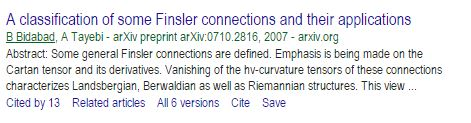
\includegraphics[height=3cm]{bidabad}
\caption{نمونه یک مقاله در گوگل اسکولار}
\end{figure}
در اینجا ما به گزینه‌ی چهارم یعنی
\lr{ Cite}
احتیاج داریم. بر روی آن کلیک کرده و پنجره‌ای مانند
\cref{fig.2}
باز می‌شود که دارای $4$ گزینه‌ی زیر است:
\begin{enumerate}
\item \lr{BibTeX}

\item \lr{EndNote}

\item \lr{RefMan}

\item \lr{RefWorks}
\end{enumerate}
\begin{figure}
\centering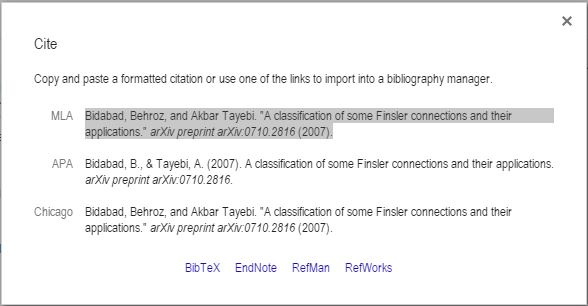
\includegraphics[scale=.6]{bibref}
\caption{پنجره‌ی باز شده در گوگل اسکولار}\label{fig.2}
\end{figure}
روی گزینه‌ی اول، یعنی
\verb;BibTeX;
کلیک کرده و همه‌ی نوشته‌های پنجره‌ی باز شده را مانند زیر، کپی کرده و در فایل
\verb;references.bib;
موجود در فایل
\verb;AUTthesis;
پیست می‌کنیم. سپس کلیدهای
\verb;Ctrl+s;
را می‌زنیم تا فایل ذخیره شود.\\
\begin{latin}
	\normalsize
\begin{verbatim}
@ article{bidabad2007classification,
title={A classification of some Finsler connections and their applications},
author={Bidabad, Behroz and Tayebi, Akbar},
journal={arXiv preprint arXiv:0710.2816},
year={2007}
}
\end{verbatim}
\end{latin}
\subsection{روش ارجاع در متن}
برای ارجاع دادن به مقاله‌ی بالا، باید در جایی که می‌خواهید ارجاع دهید، دستور زیر را تایپ کنید:
\begin{latin}
\lr{$\backslash$cite\{bidabad2007classification\}}
\end{latin}
همانطور که مشاهده می‌کنید از کلمه‌ای که در سطر اول ادرس مقاله آمده (یعنی کلمه‌ی پس از
\lr{@article$\lbrace$})
استفاده کرده‌ایم. پس از دستور فوق، به صورت \cite{bidabad2007classification} و \cite{aa} مرجع خواهد خورد. توجه شود که در صورتی مراجع چاپ خواهند شد که در متن به انها ارجاع داده شده باشد. همچنین برای ارجاع چندتایی از دستور 
\lr{$\backslash$cite\{name1, name2,...\}}
استفاده کنید که به‌صورت \cite{najafi2008finsler, zakeri, najafi} ارجاع خواهند خورد.
\subsection{روش اجرای برنامه}
ابتدا فایل
\verb;AUT_thesis.tex;
را باز کرده و آن را دو بار اجرا کنید. سپس حالت اجرا را از 
\verb;Build Quick;
به حالت
\verb;Bibtex;
تغییر داده و دوباره برنامه را اجرا کنید. دو بار دیگر برنامه را در حالت 
\verb;Build Quick;
اجرا کرده و نتیجه را مشاهده کنید. در این روش تمامی مراجع بر اساس اینکه کدام یک در متن زودتر به آن ارجع داده شده لیست خواهند شد.
\subsection{مراجع فارسی}
برای نوشتن مراجع فارسی باید به صورت دستی، در همان فایل قبلی به صورت زیر عمل می‌کنیم:
\begin{LTR}
\noindent\verb;@article{manifold,;\\
\verb;title={;منیفلد هندسه\verb;},;\\
\verb;author={;بیدآباد دکتربهروز \verb;},;\\
\verb;journal{; امیرکبیر صنعتی دانشگاه\verb;},;\\
\verb;year={1389},;\\
\verb;LANGUAGE={Persian};\\
\verb;};
\end{LTR}
همانطور که مشاهده می‌کنید تنها تفاوت آن با حالت مراجع انگلیسی، سطر آخر آن می‌باشد که زبان را مشخص می‌کند که حتماً باید نوشته شود.
\section{راهنمای واژه‌نامه}

به دلیل پیچیدگی واژه‌نامه‌های موجود در سایت پارسی لاتک، از روش زیر برای نوشتن واژه‌نامه استفاده کنید:

ابتدا با استفاده از اکسل، واژه های خود را یک‌بار براساس حروف الفبای فرسی و بار دیگر انگلیسی مرتب کنید. سپس واژه ها را در فایل \lr{dicen2fa} و \lr{dicfa2en} قرار دهید.

\section{ساخت نمایه}\label{Namaye}
\subsection{ساخت نمایه}
 \begin{enumerate}

\item
کلمات مورد نظر خود مثلا \lr{word} با دستور \verb|\index{word}| ایندکس کنید.
\item
نحوه‌ی اجرای \lr{Make Index}   در ویرایشگرهای \lr{TeX Maker} و \lr{TeX Works}:
\begin{itemize}
\item  تک‌میکر: از منوی \lr{Tools} گزینه‌ی \lr{Xindy Make Index} را کلیک کنید یا از دکمه‌‌های میانبر \lr{Ctrl+Alt+I} استفاده کنید.

\item  تک‌ورکز: ابتدا باید مثل عکس زیر تنظیم  و سپس گزینه‌ی \lr{Xindy Make Index}  انتخاب و روی دکمه‌ی سبز رنگ کلیک کنید یا از دکمه‌های  \lr{Ctrl+T} استفاده کنید.

\begin{figure}[!h]
\centerline{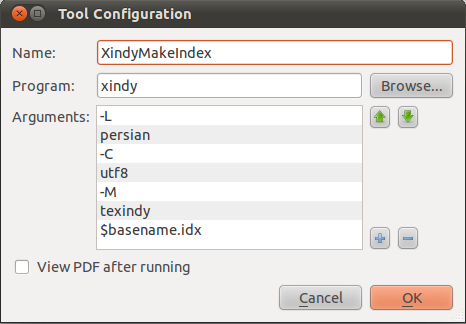
\includegraphics[width=.5\textwidth]{Xindy_Make_Index.png}}
\caption{تنظیمات مربوط به تک‌ورکز}
\end{figure}

\end{itemize}
 \end{enumerate}
 
 \index{کتاب}
\index{پارسی‌لاتک}
\index{بی‌دی}
\index{سوال}
\index{عنصر}
\index{گزینه}
\index{ژاکت}
\index{مرکز دانلود}
\index{اجرا}
\index{تک‌لایو}
\index{ثالث}
\index{جهان}
\index{چهار}
\index{حمایت}
\index{خواهش}
\index{دنیا}
\index{زی‌پرشین}
\index{ریحان}
\index{شیرین}
\index{صمیمی}
\index{ضمیر}
\index{طبیب}~
را در فایل 
\verb~AUTthesis.tex~،
غیرفعال%
\RTLfootnote{
برای غیرفعال کردن یک دستور، کافی است پشت آن، یک علامت
\%
 بگذارید.
}
 کنید. زیرا در غیر این صورت، ابتدا مطالب فصل ۱ و ۲ پردازش شده (که به درد ما نمی‌خورد؛ چون ما می‌خواهیم خروجی فصل ۳ را ببینیم) و سپس مطالب فصل ۳ پردازش می‌شود و این کار باعث طولانی شدن زمان اجرا می‌شود. زیرا هر چقدر حجم فایل اجرا شده، بیشتر باشد، زمان بیشتری هم برای اجرای آن، صرف می‌شود.

\subsection{مراجع}
برای وارد کردن مراجع به فصل 2
مراجعه کنید.
\subsection{واژه‌نامه فارسی به انگلیسی و برعکس}
برای وارد کردن واژه‌نامه فارسی به انگلیسی و برعکس، بهتر است مانند روش بکار رفته در فایل‌های 
\verb;dicfa2en;
و
\verb;dicen2fa;
عمل کنید.

\section{اگر سوالی داشتم، از کی بپرسم؟}
برای پرسیدن سوال‌های خود در مورد حروف‌چینی با زی‌پرشین،  می‌توانید به
 \href{http://forum.parsilatex.com}{تالار گفتگوی پارسی‌لاتک}%
\LTRfootnote{\url{http://www.forum.parsilatex.com}}
مراجعه کنید. شما هم می‌توانید روزی به سوال‌های دیگران در این تالار، جواب بدهید.
